% !TEX root = ../main.tex

\section{Entrained flow reactor (EFR)}

The following sections provide geometric dimensions and process flow information for the entrained flow reactor (EFR). Computational model results are also presented in this section.

\subsection{Experimental setup}

Fast pyrolysis in the TCPDU system occurs in the entrained flow reactor (pictured in Figure \ref{fig:efr-assembly}) which is comprised of a series of horizontal and vertical pipes connected with 90 degree elbows. Dimensions and material information about the EFR are provided in Figure \ref{fig:efr-geometry} below. Operating conditions such as temperatures, pressures, and flow rates for the EFR are shown in Figure \ref{fig:efr-flow}. Nitrogen gas at 500$^{\circ}$C is used as the conveying medium for the solids.

\begin{figure}[!ht]
	\centering
	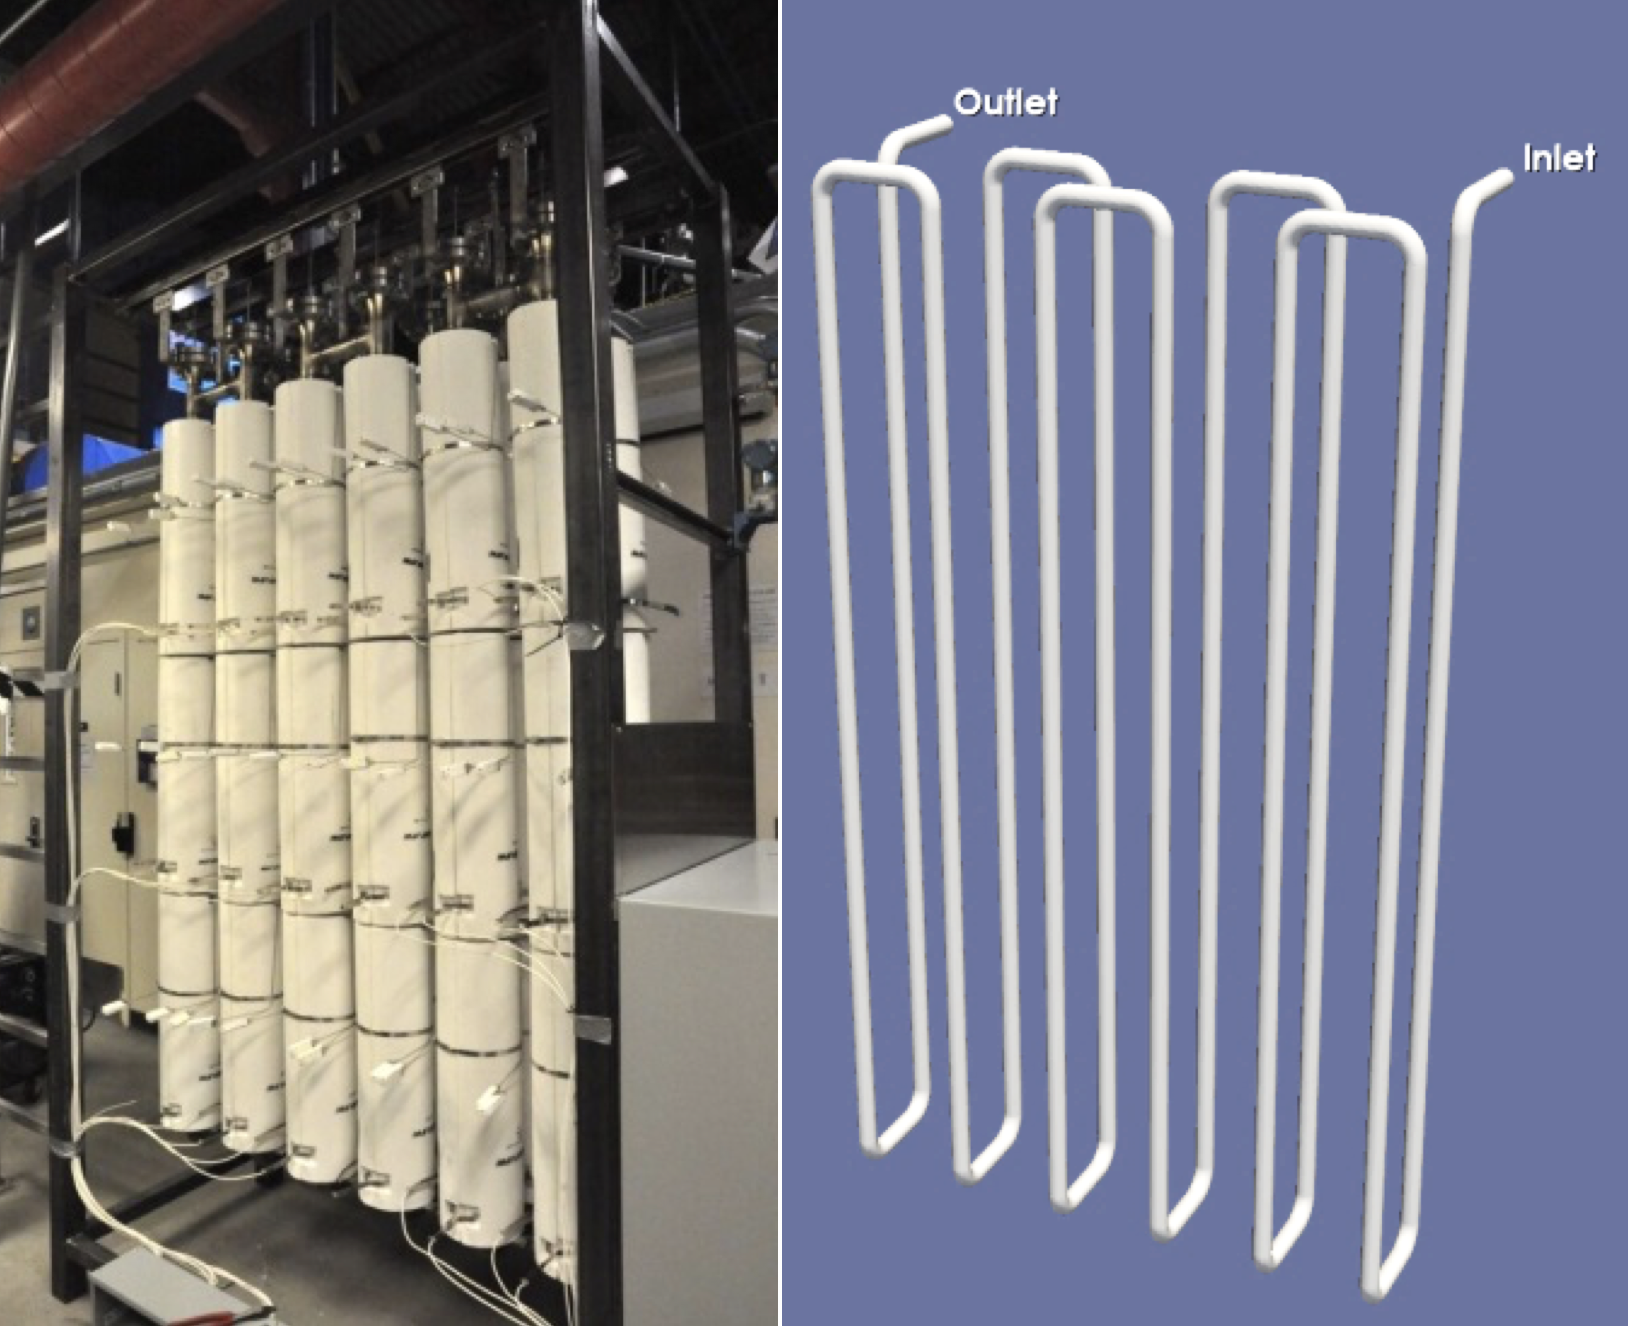
\includegraphics[width=0.8\textwidth]{figures/efr-assembly.png}
	\caption{Left - picture of the EFR assembly with heat jackets, insulation, and thermocouples. Right - CAD representation of the EFR pipe assembly used for MFiX simulations.}
	\label{fig:efr-assembly}
\end{figure}

\begin{figure}[!ht]
	\centering
	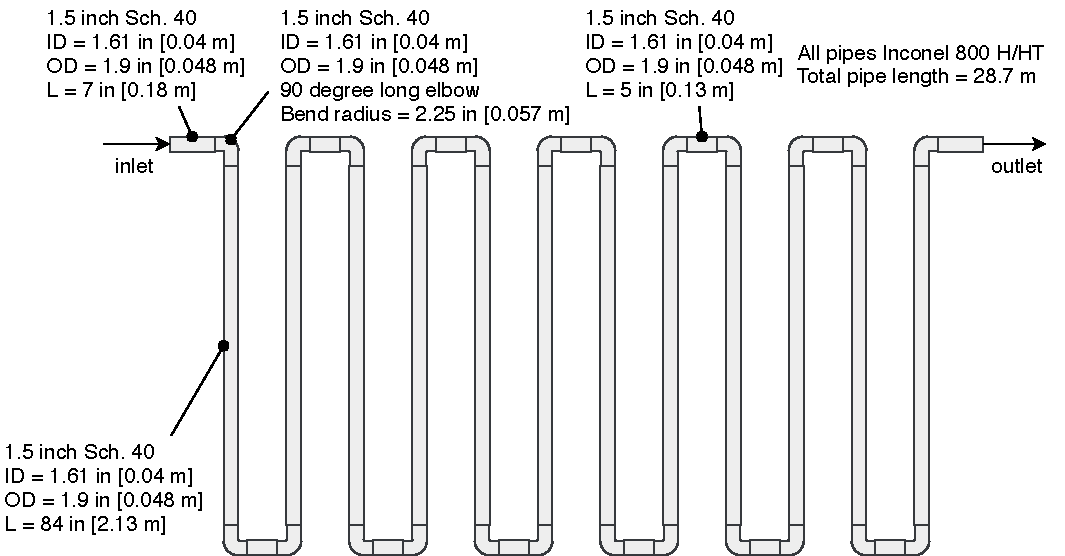
\includegraphics[width=0.8\textwidth]{figures/efr-geometry.pdf}
	\caption{Geometry of the entrained flow reactor at NREL.}
	\label{fig:efr-geometry}
\end{figure}

\begin{figure}[!ht]
	\centering
	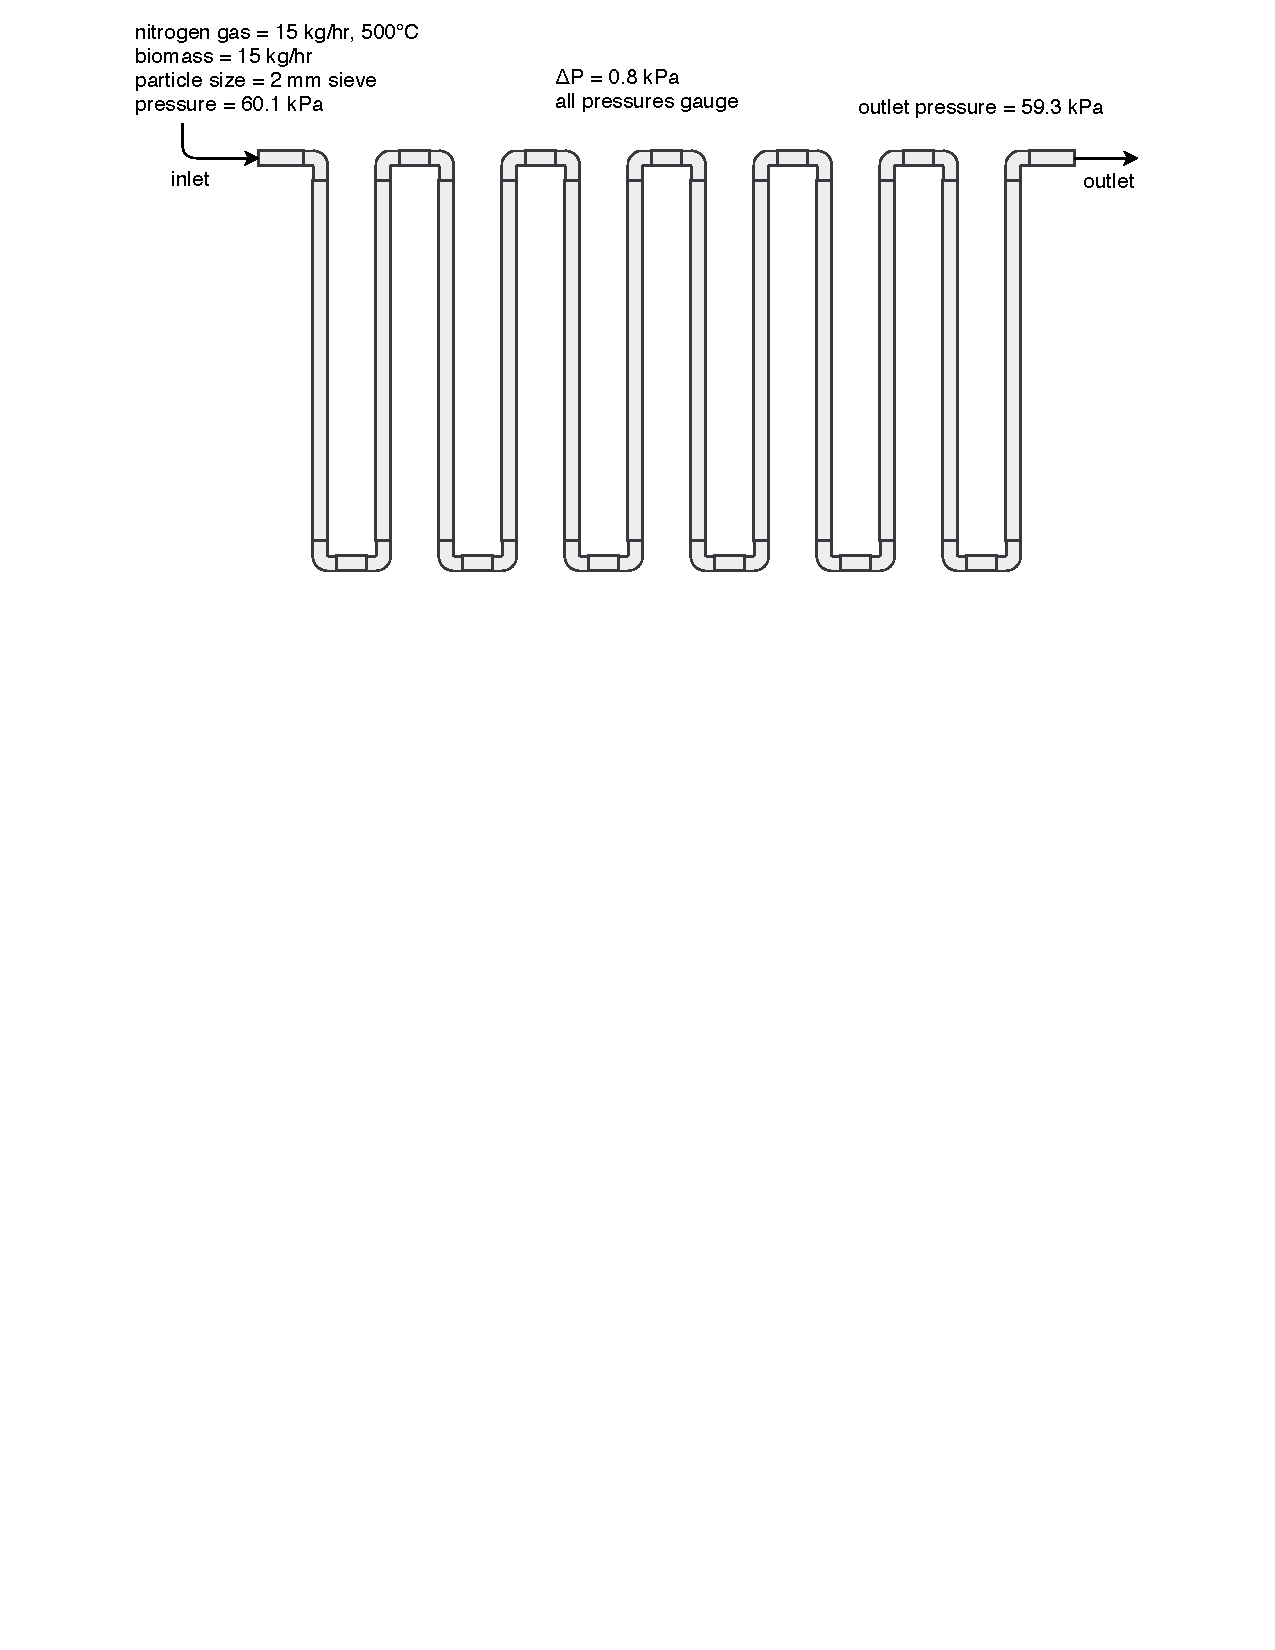
\includegraphics[width=\textwidth]{figures/efr-flow.pdf}
	\caption{Typical operating conditions for the entrained flow reactor.}
	\label{fig:efr-flow}
\end{figure}

\subsection{Residence time distribution}

Ideally, experimental measurements are used to develop a residence time distribution (RTD) curve of the solids in a fluidized system. However, the reactor systems at NREL are not equipped to measure solids residence time therefore computational reactor models were developed to determine this information for the particle-scale simulations. The residence time distributions were determined from MFiX simulations of spheres at various particle sizes with a {$\text{N}_2$} carrier gas velocity of 4.78 m/s and a solids mass flow rate of 15 kg/s. The EFR is essentially a pneumatic conveyor where biomass particles flow through a long pipe with several bends. The CAD representation of the EFR used for the MFiX residence time simulations is shown in Figure \ref{fig:efr-assembly}.

By using a discrete element model (DEM) in MFiX we can track individual particles in the reactor and determine when they leave the system. The DEM simulation was populated with two thousand particles comprised of five different sizes that were initially placed at the inlet of the reactor to simulate a pulse-tracer experiment. An initial gas flow rate and pressure drop are imposed along the reactor to allow the system to quickly attain steady state conditions. A gas phase boundary condition is established at the reactor entrance pushing 15 kg/hr of hot nitrogen gas through the system to reach solids fluidization. A pressure outlet boundary condition was set up at the reactor exit to allow particles and gas to flow out of the system. The particles are tracked as they move over time and their reactor exit time is recorded. The DEM simulation with particles after three seconds in the reactor is shown in Figure \ref{fig:mfix-particles}.

\begin{figure}[!ht]
	\centering
	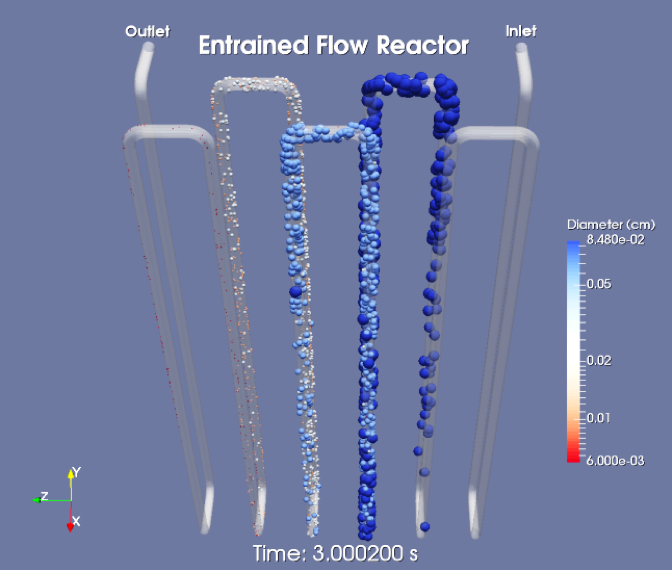
\includegraphics[width=0.6\textwidth]{figures/mfix-particles.png}
	\caption{Entrained flow reactor after approximately three seconds. Particle diameters are scaled 50x for visualization purposes.}
	\label{fig:mfix-particles}
\end{figure}

After simulation setup, it takes approximately four weeks of computation time on a single-core machine for all particles to leave the reactor. Using the recorded exit time of each particle, the concentration of particles exiting the reactor at a given time step is calculated. From this information, a concentration profile and associated exit age distribution for a given particle size distribution is developed for the EFR. The concentration and residence time distribution curve for the solids in the entrained flow reactor is shown in Figure \ref{fig:mfix-restime}. It should be noted that at the time of this report, simulations using the particle measurements from Microtrac were still running. Therefore, to improve the results of the particle-scale pyrolysis model, the revised RTD should be incorporated into future models.

\begin{figure}[!ht]
	\centering
	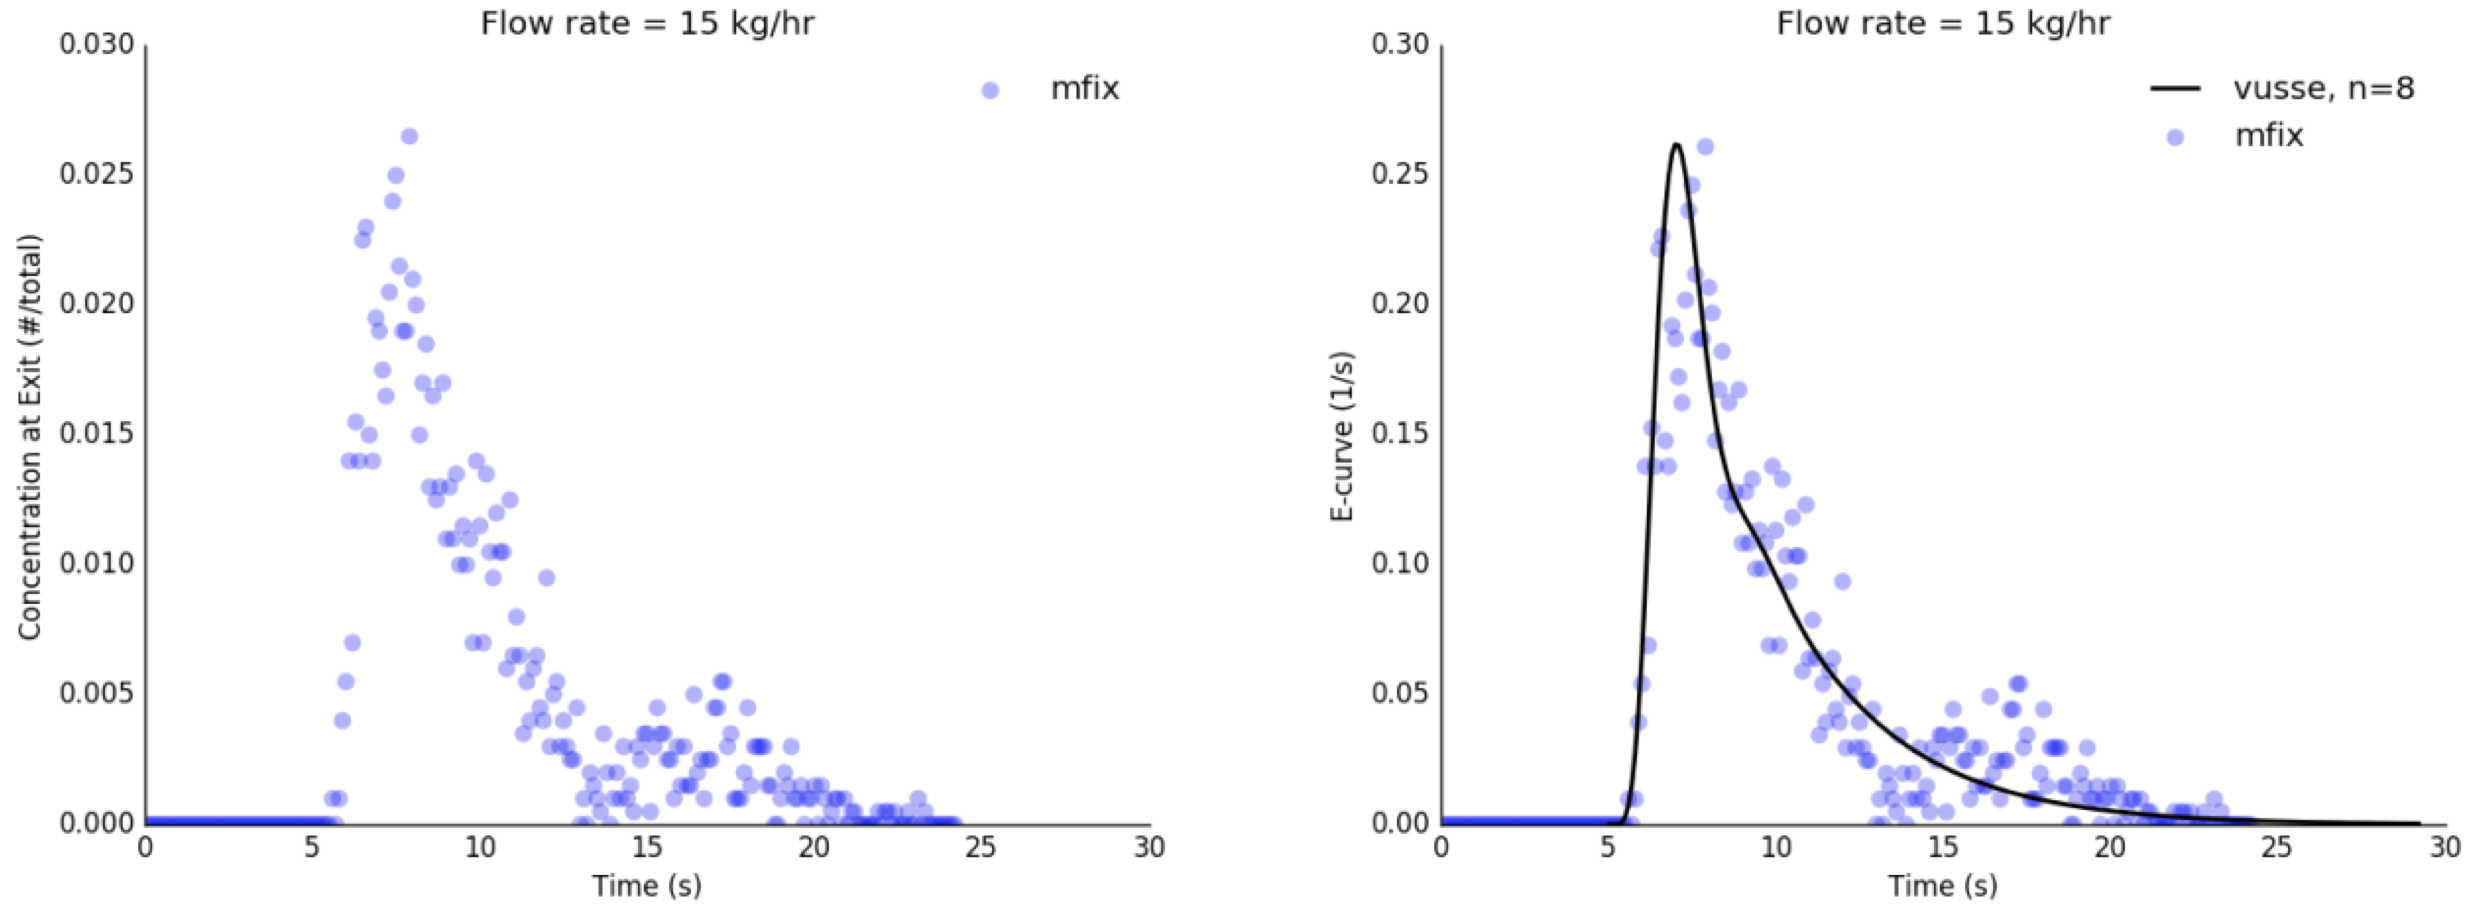
\includegraphics[width=\textwidth]{figures/mfix-restime.png}
	\caption{Concentration of oak particles leaving EFR (left). Residence time distribution calculated from concentration profile (right). Reactor conditions 500$^{\circ}$C with 15 kg/s solids and gas flow. The solid line (right) represents the Van de Vusse correlation for estimating the number of CSTRs that represent mixing in the system.}
	\label{fig:mfix-restime}
\end{figure}

\subsection{Biomass pyrolysis kinetics}

The Ranzi et al. kinetic scheme for biomass fast pyrolysis is described in this section.

\begin{table}[H]
	\centering
	\caption{Solid species in Ranzi kinetic scheme.}
	\begin{tabular}{@{}clll@{}}
		\toprule
		Item & Abbreviation & Name & Formula \\
		\midrule
		1  	& CELL 		& cellulose 					& C$_6$H$_{10}$O$_5$ \\
		2 	& CELLA 	& activated cellulose			& C$_6$H$_{10}$O$_5$ \\
		3 	& CHAR		& char 						  	& C \\
		4 	& GCO 		& metaplastic carbon monoxide 	& CO \\
		5 	& GCO2 		& metaplastic carbon dioxide  	& CO$_2$ \\
		6 	& GCH4		& metaplastic methane			& CH$_4$ \\
		7  	& GC2H4		& metaplastic ethylene			& C$_2$H$_4$ \\
		8 	& GCH3OH	& metaplastic methyl alcohol  	& CH$_4$O \\
		9 	& GCOH2		& metaplastic formaldehyde	  	& CH$_2$O \\
		10	& GH2 		& metaplastic hydrogen 		  	& H$_2$ \\
		11  & GMSW 		& hemicellulose softwood 		& C$_5$H$_8$O$_4$ \\
		12 	& HCE1 		& hemicellulose 		 		& C$_5$H$_8$O$_4$ \\
		13 	& HCE2 		& hemicellulose 		 		& C$_5$H$_8$O$_4$ \\
		9 	& HMWL		& heavy molecular weight lignin	& C$_{24}$H$_{28}$O$_4$ \\
		14  & LIG 		& lignin 				 		& C$_{11}$H$_{12}$O$_4$ \\
		15 	& LIGC 		& lignin carbon 		 		& C$_{15}$H$_{14}$O$_4$ \\
		16 	& LIGCC 	& lignin carbon 		 		& C$_{15}$H$_{14}$O$_4$ \\
		17 	& LIGH 		& lignin hydrogen 		 		& C$_{22}$H$_{28}$O$_9$ \\
		18 	& LIGO 		& lignin oxygen 		 		& C$_{20}$H$_{22}$O$_{10}$ \\
		19 	& LIGOH		& lignin hydroxide 		 		& C$_{19}$H$_{22}$O$_8$ \\
		20	& XYHW 		& hemicellulose hardwood 		& C$_5$H$_8$O$_4$ \\
		\bottomrule
	\end{tabular}
\end{table}

\begin{table}[H]
	\centering
	\caption{Gas species in Ranzi kinetic scheme.}
	\begin{tabular}{@{}clll@{}}
		\toprule
		Item & Abbreviation & Name & Formula \\
		\midrule
		1	& ACAC 		& acetic acid 				& C$_2$H$_4$O$_2$ \\
		2 	& ALD3 		& propanal 					& C$_3$H$_6$O \\
		3 	& ANISOLE 	& anisole 					& C$_7$H$_8$O \\
		4 	& C2H4 		& ethylene 					& C$_2$H$_4$ \\
		5 	& C2H6 		& ethane 					& C$_2$H$_6$ \\
		6 	& C2H5OH 	& ethanol 					& C$_2$H$_6$O \\
		7 	& C2H3CHO 	& 2-propenal				& C$_3$H$_4$O \\
		8 	& C3H6O2 	& propanal, 3-hydroxy-		& C$_3$H$_6$O$_2$ \\
		9  	& CH2O 		& formaldehyde 				& CH$_2$O \\
		10 	& CH3OH 	& methyl alcohol 			& CH$_4$O \\
		11 	& CH3CHO 	& acetaldehyde 				& C$_2$H$_4$O \\
		12  & CH4 		& methane 					& CH$_4$ \\
		13  & CO 		& carbon monoxide 			& CO \\
		14  & CO2 		& carbon dioxide 			& CO$_2$ \\
		15  & COUMARYL 	& coumaryl alcohol 			& C$_9$H$_{10}$O$_2$ \\
		16 	& FE2MACR 	& sinapaldehyde 			& C$_{11}$H$_{12}$O$_4$	\\
		17 	& FURF 		& furfural 					& C$_5$H$_4$O$_2$	\\
		18 	& GLYOX 	& glyoxal				 	& C$_2$H$_2$O$_2$ \\
		19	& H2 		& hydrogen 				 	& H$_2$ \\
		20	& H2O 		& water 				 	& H$_2$O \\
		21 	& HAA 		& hydroxy-acetaldehyde 		& C$_2$H$_4$O$_2$ \\
		22  & HCOOH 	& formic acid 			 	& CH$_2$O$_2$ \\
		23  & HMFU		& 5-hydroxymethyl-furfural	& C$_6$H$_6$O$_3$ \\
		24 	& LVG		& levoglucosan 			 	& C$_6$H$_{10}$O$_5$ \\
		25	& PHENOL 	& phenol 				 	& C$_6$H$_6$O \\
		26 	& XYLAN 	& xylosan 				 	& C$_5$H$_8$O$_4$ \\
		\bottomrule
	\end{tabular}
\end{table}
